\chapter{The Classical Banach Spaces}
\begin{rmk}%117
	We explore briefly one major application of the Lebesgue integral. 
	First I recall some familiar definitions. 
\end{rmk}

\begin{defn}\label{d:metricspace}%118
	A \textbf{metric space} is a pair $(X, d)$ where $X$ is a set 
	and $d: X \times X \rightarrow \R$ is a function such that 
	\begin{enumerate}[(a)]
	\item $d(x, y) \ge 0$ for all $x, y \in X$ and $d(x,y) = 0$ iff $x = y$. 
	\item $d(x, y) = d(y, x)$ for all $x, y \in X$. 
	\item $d(x, z) \le d(x, y) + d(y, z)$ for all $x, y, z \in X$.
	\end{enumerate}
\end{defn}

\begin{defn}~%119
	\begin{enumerate}
	\item A sequence $\{x_n\}_{n=1}^\infty$ \textbf{converges to the limit} 
		$x$ in the metric space $(X,d)$ if for every $\epsilon > 0$ there is an 
		integer $N$ such that $d(x_n,x) < \epsilon$ whenever $n \ge N$. 
	\item A sequence $\{x_n\}_{n=1}^\infty$ is a \textbf{Cauchy sequence} 
		in the metric space $(X,d)$ if for every $\epsilon > )$ there is an 
		integer $N$ such that $d(x_n,x_m) < \epsilon$ whenever $m,n \ge N$. It 
		is easy to see that every convergent sequence is Cauchy, but the converse 
		is in general not true. 
	\item A metric space $(X,d)$ is \textbf{complete} if every Cauchy sequence 
		is convergent. 
	\end{enumerate}
\end{defn}

\begin{rmk}%120
	You will recall that the set of rationals $\Q$ with the usual distance on $\R$ 
	is not complete, but $\R$ is complete, since ``the holes have been filled in.'' 
	A somewhat different example is that the open interval (0,1) with the usual 
	distance is not complete, because sequences ``converging to 0 or 1'' do not 
	have a limit. In each case we know how to find the complete metric space that 
	appears to contain the given metric space most efficiently. You may have seen 
	a general procedure to produce the ``completion'' of any metric space-the idea 
	is that the points of the completion are equivalence classes of Cauchy sequences 
	of points of the original space. Constant sequences may be identified with 
	points of the original space, so we can think of this as a larger space. It is 
	rather hard to visualize this abstract completion, so more concrete constructions 
	(as in the two examples) are desirable. The Lebesgue integral will provide some 
	of these. 
\end{rmk}

\pagebreak
\begin{ex}~%121
	\begin{enumerate}
	\item Any non-empty subset of $\R^n$ together with the usual Euclidean distance 
		is a metric space. It is also possible to introduce alternative distance 
		functions, such as $d_1(x,y) = \sum\limits_{j=1}^n|x_j-y_j|$ for 
		$x=(x_1,...,x_n)$, $y=(y_1,...,y_n)$ in $\R^n$. It turns out that these 
		are not very different in the sense that a sequence converges with respect 
		to any readsonable distance function in $\R^n$ (such as $d_1$) if and only 
		if it converges to the same limit with respect to the Euclidean distance.
	\item The set $C[0,1]$ of all real-valued continuous functions on $[0,1]$ is a 
		metric space with the distance $d(f,g) = \max\limits_{x}|f(x)-g(x)|$. 
		(Since the set $[0,1]$ is compact, the supremum of the differences 
		$|f(x)-g(x)|$ is actually a max.) Convergence with respect to this distance 
		is uniform convergence. The theorem that the limit of a uniformly convergent 
		sequence of continuous functions is continuous translates in this terminology 
		to the statement that $C[0,1]$ with this metric is a complete metric space. 
		However for the set $C[0,1]$ it is easy to define other distance functions 
		which are essentially different in the sense that they produce a form of 
		convergence that is not equivalent to uniform convergence and with repsect to 
		which $C[0,1]$ is not a complete metric space. We will do this shortly. 
	\end{enumerate}
\end{ex}

\begin{defn} %122
	A real \textbf{linear space} (or real \textbf{vector space}) is a triple 
	$(V,+,\cdot)$ consisting of a set $V$ of objects (called \textbf{vectors}) a 
	mapping $+:V\times V\rightarrow V$ (called \textbf{addition}) and a mapping 
	$\cdot : \R \times V \rightarrow V$ (called \textbf{scalar multiplication}) 
	such that 
	\begin{enumerate}
	\item $u + v = v + u$ for all $u, v \in V$, 
	\item $(u + v) + w = u + (v + w)$ for all $u, v, w \in V$, 
	\item there is a vector $0 \in V$ (called the \textbf{zero vector}) such that 
		$u + 0 = u$ for all $u \in V$,
	\item for each $u \in V$ there is a vector $-u \in V$ such that $u + (-u) = 0$, 
	\item $c(u + v) = cu + cv$ for all $u, v \in V$ and all $c \in \R$, 
	\item $(c + d)u = cu = du$ for all $u \in V$ and all $c, d\in \R$,  
	\item $c(du) = (cd)u$ for all $c, d \in \R$ and all $u \in V$, 
	\item $1u = u$ for all $u \in V$. 
	\end{enumerate}
\end{defn}

\begin{defn}%123
	A subset $W$ of a vector space $V$ is a \textbf{subspace} of $V$ if it is a 
	vector space in its own right with the same operations as $V$. 
\end{defn}

\pagebreak
\begin{ex}~ %124
	\begin{enumerate}
	\item Once again $\R^n$ with the obvious component-wise operations is the 
		basic example. This time, however, only certain subsets are subspaces 
		of $\R^n$. (Those consisting of lines or planes through the origin, or 
		just the zero element for $n = 3$.)
	\item $C[0,1]$ is also a vector space with the usual operations of adding functions 
		and multiplying a function by a real number. The set $\Sp$ of of polynomial 
		functions is a subspace of $C[0,1]$, and for every positive integer $n$, 
		the set $\Sp_n$ of polynomials of degree at most $n$ is a subspace of $\Sp$.  
	\end{enumerate}
\end{ex}

\begin{defn}%125
	A \textbf{normed linear space} is a pair $(V, \|\cdot\|)$ consisting of a real 
	linear space $V$ (strictly $(V,+,\cdot)$) and a mapping $\|\cdot\|:v\rightarrow \R$ 
	called a \textbf{norm} on $V$ such that 
	\begin{enumerate}
	\item $\|x\|\ge 0$ for all $x\in V$ and $\|x\|=0$ if and only if $x = 0$ (the zero 
		element of $V$)
	\item $\|x+y\|\le\|x\|+\|y\|$ for all $x,y\in V$. 
	\end{enumerate}
\end{defn}

\begin{rmk} %126
	A normed linear space is a metric space with the distance function $d(x,y) = \|x-y\|$. 
\end{rmk}

\begin{defn}%127
	A normed linear space that is a complete metric space with this distance function is 
	called a \textbf{Banach space}. 
\end{defn}

\begin{ex}%128
	$C[0,1]$ with the norm $\|f\|=\max\limits_{x}|f(x)|$ is a Banach space. So is $\R^n$ 
	with the Euclidean norm or, for that matter, any other reasonable norm. 
\end{ex}

\begin{pblm} \label{p:129} %129
	Let $\phi$ be a continuous, increasing, real-valued function defined on $[0,\infty)$ 
	such that $\phi(0) = 0$ and $\lim\limits_{x\to\infty}\phi(x) = \infty$. Let 
	$\varPsi$ be the inverse of $\phi$. Let 
	$\Phi(x) = \int_0^x\phi$ and $\Psi(x) = \int_0^x\varPsi$. Then for any positive real 
	numbers $a$ and $b$, 
	\begin{equation*}
		ab \le \Phi(a) + \Psi(b)
	\end{equation*}
	with equality if and only if $b = \phi(a)$. \\
	{\scriptsize{(interpret $\Phi(a)$ and $\Phi(b)$ as areas associated with the graph of 
	$\phi$. For $\Psi(b)$ you will need to remember that the graph of $\varPsi$ is the 
	``mirror image'' of the graph of $\phi$, so you can find $\Psi(b)$ as an area between 
	the $y$-axis and the graph of $\phi$. This result is called Young's Inequality.)}}
\pagebreak
\begin{proof}
	Note first that since $\phi$ is non-decreasing, and is a well-defined function such 
	that its inverse is $\psi$, then $\psi$ is also non-decreasing. 

	\begin{itemize}
	\item $\psi(b) = a$: Then since $\psi$, $\phi$ are inverses, this means that $\phi(a) = b$, and 
	so $ab = \Phi(a) + \Psi(b)$
	\begin{center}
	\resizebox{0.3\textwidth}{!}{
		\begin{tikzpicture}
		\begin{axis}[
				xmin = -5.5, xmax = 5.5, ymin = -5.5, ymax = 5.5, 
				grid = both, axis lines = middle, 
				grid style={line width=.1pt, draw=gray!30}, 
				xticklabels={,,},
				yticklabels={,,},
				minor tick num=1,
				major grid style={line width=.2pt, draw=gray!60} 
			]
			\addplot[name path=xaxis, draw=none, domain=0:26,samples=10]{0};
			\addplot[name path=yaxis, draw=none, ] coordinates{(0.0, 4.0) (4.0, 4.0)};
			\addplot[name path=phi, line width=0.5pt,domain=0.0:25.5,samples=500, mark=none,color=red]{2.0 * sqrt(x)};
			\addplot[name path=psi, line width=0.5pt,domain=0.0:25.5,samples=500, mark=none,color=blue]{ 0.25 * x*x };
			\draw (axis cs:5.2,4.3) node[color=red] {$\phi$};
			\draw (axis cs:4.3,5.2) node[color=blue] {$\varPsi$};
		\end{axis}
		\end{tikzpicture}
	}
	~
	\resizebox{0.3\textwidth}{!}{
		\begin{tikzpicture}
		\begin{axis}[
				xmin = -5.5, xmax = 5.5, ymin = -5.5, ymax = 5.5, 
				grid = both, axis lines = middle, 
				grid style={line width=.1pt, draw=gray!30}, 
				xticklabels={,,},
				yticklabels={,,},
				minor tick num=1,
				major grid style={line width=.2pt, draw=gray!60} 
			]
			\addplot[name path=xaxis, draw=none, domain=0:26,samples=10]{0};
			\addplot[name path=yaxis, draw=none, ] coordinates{(0.0, 4.0) (4.0, 4.0)};
			\addplot[name path=phi, line width=0.5pt,domain=0.0:25.5,samples=500, mark=none,color=red]{2.0 * sqrt(x)};
			\addplot[name path=psi, line width=0.5pt,domain=0.0:25.5,samples=500, mark=none,color=blue]{ 0.25 * x*x };
			\draw (axis cs:5.2,4.3) node[color=red] {$\phi$};
			\draw (axis cs:4.3,5.2) node[color=blue] {$\varPsi$};
			\addplot[fill=red ,opacity=0.3]fill  between[of=phi and xaxis, soft clip={domain=0:4}];
			\addplot[fill=blue,opacity=0.3]fill  between[of=phi and yaxis, soft clip={domain=0:4.0}];
			\draw (axis cs:4,-.6) node[color=red] {$a$};
			\draw (axis cs:-.5,4) node[color=blue] {$b$};
			\draw (axis cs:-1.4,4) node[color=red ] {$\phi(a)$};
			\draw (axis cs:4,-1.4) node[color=blue] {$\psi(b)$};
			\draw[fill, pattern=north east lines, pattern color=black, draw=none,opacity=0.5] (axis cs:0,0) rectangle (axis cs:4,4);
			\draw (axis cs:2.5,3) node[color=black,opacity=0.8] {$ab$};
		\end{axis}
		\end{tikzpicture}
	}
	\end{center}

	\item $\psi(b) < a$: Note that this implies that $\phi(a) > b$, and so (using both facts), 
	$\Phi(a) - \Phi(\psi(b)) > b(a - \psi(b))$. 

	$ab = \Phi(\psi(b)) + \Psi(b) + b(a - \psi(b))$
	\begin{center}
	\resizebox{0.28\textwidth}{!}{
	\begin{tikzpicture}
	\begin{axis}[
			xmin = -5.5, xmax = 15.5, ymin = -5.5, ymax = 15.5, 
			grid = both, axis lines = middle, 
			grid style={line width=.1pt, draw=gray!30}, 
			xticklabels={,,},
			yticklabels={,,},
			minor tick num=1,
			major grid style={line width=.2pt, draw=gray!60} 
		]
		\addplot[name path=xaxis, draw=none, domain=0:26,samples=10]{0};
		\addplot[name path=yaxis, draw=none, ] coordinates{(0.0, 6.0) (9.0, 6.0)};
		\addplot[name path=phi,line width=0.5pt,domain=0.0:25.5,samples=500,mark=none,color=black]{2.0 * sqrt(x)};
		%
		\draw (axis cs:15,7.0) node[color=black] {$\phi$};
		\draw (axis cs:12,-.6) node[color=red] {$a$};
		\draw (axis cs:-.5,6) node[color=blue] {$b$};
		\draw (axis cs:9,-.6) node[color=blue] {$\psi(b)$};
		%
		\addplot [dashed,color=blue] coordinates { (9, 6) (9, 0) };
		\addplot[pattern=north west lines, pattern color=blue,opacity=0.5] fill between[of=yaxis and phi,soft clip={domain=0:9}];
		\addplot[pattern=north east lines, pattern color=blue,opacity=0.5] fill between[of=phi and xaxis,soft clip={domain=0:9}];
		\addplot[color=black,opacity=0.5] fill between[of=phi and xaxis,soft clip={domain=9:12}];
		\draw[fill,pattern=grid, pattern color=red,opacity=0.5] (axis cs:9,0) rectangle (axis cs:12,6);
		\draw[fill=none,color=blue] (axis cs:0,0) rectangle(axis cs:9,6);
		\draw[fill=none,color=red] (axis cs:9,0) rectangle(axis cs:12,6);
		%
		\draw (axis cs:0.5,-3) node[color=blue] {$\Phi(\psi(b)) + \Psi(b)$};
		\draw (axis cs:11.0,-3) node[color=red] {$b(a - \psi(b))$};
		\draw (axis cs:8.0,10) node[color=black] {$\Phi(a) - \Phi(\psi(b))$};
		\draw [->, blue  ] (axis cs:0.5, -2) -- (axis cs:1.0, -.2);
		\draw [->, red   ](axis cs:11.0, -2) -- (axis cs:10.5, -.2);
		\draw [->, black ](axis cs:7.5, 9.2) -- (axis cs:10.5, 6.5);
	\end{axis}
	\end{tikzpicture}
	}
	~
	\resizebox{0.28\textwidth}{!}{
	\begin{tikzpicture}
	\begin{axis}[
			xmin = -5.5, xmax = 15.5, ymin = -5.5, ymax = 15.5, 
			grid = both, axis lines = middle, 
			grid style={line width=.1pt, draw=gray!30}, 
			xticklabels={,,},
			yticklabels={,,},
			minor tick num=1,
			major grid style={line width=.2pt, draw=gray!60} 
		]
		\addplot[name path=xaxis, draw=none, domain=0:26,samples=10]{0};
		\addplot[name path=yaxis, draw=none, ] coordinates{(0.0, 6.0) (9.0, 6.0)};
		\addplot[name path=phi,line width=0.5pt,domain=0.0:25.5,samples=500,mark=none,color=red]{2.0 * sqrt(x)};
		\draw (axis cs:15,7.0) node[color=red] {$\phi$};
		\addplot[fill=red ,opacity=0.3]fill between[of=phi and xaxis,soft clip={domain=0:12}];
		\addplot[fill=blue,opacity=0.3]fill between[of=phi and yaxis,soft clip={domain=0:9.0}];
		\draw (axis cs:12,-.6) node[color=red] {$a$};
		\draw (axis cs:-.5,6) node[color=blue] {$b$};
		\draw[fill,pattern=grid,pattern color=black,opacity=0.5] (axis cs:0,0) rectangle (axis cs:12,6);
		\draw (axis cs:6,3) node[color=black,opacity=0.8] {$ab$};
	\end{axis}
	\end{tikzpicture}
	}
	\end{center}

	\item $\psi(b) > a$: Note that this implies that $\phi(a) < b$, and so (similarly to the case above), 
	$\Psi(b) - \Psi(\phi(a)) > a(b - \phi(a))$. 

	\begin{center}
	\resizebox{0.27\textwidth}{!}{
	\begin{tikzpicture}
	\begin{axis}[
			xmin = -5.5, xmax = 15.5, ymin = -5.5, ymax = 15.5, 
			grid = both, axis lines = middle, 
			grid style={line width=.1pt, draw=gray!30}, 
			xticklabels={,,},
			yticklabels={,,},
			minor tick num=1,
			major grid style={line width=.2pt, draw=gray!60} 
		]
		\addplot[name path=xaxis, draw=none, domain=0:26,samples=10]{0};
		\addplot[name path=yaxis, draw=none, ] coordinates{(0.0, 6.0) (9.0, 6.0)};
		\addplot[name path=yaxis2, draw=none, ] coordinates{(0.0, 4.0) (4.0, 4.0)};
		\addplot[name path=psi, line width=0.5pt,domain=0.0:25.5,samples=500, mark=none,color=black]{ 2.0 * sqrt(x)};%0.25 * x*x };
		%
		\draw (axis cs:15.0,7) node[color=black] {$\Phi$};
		\draw (axis cs:4,-.6) node[color=red] {$a$};
		\draw (axis cs:-1.5,6) node[color=blue] {$b$};
		\draw (axis cs:-1.5,4) node[color=red] {$\phi(a)$};
		%
		\addplot[color=black,opacity=0.5] fill between[of=yaxis and psi,soft clip={domain=4:9}];
		\draw[fill, color=black, opacity=0.5] (axis cs:0,4) rectangle(axis cs:4, 6);
		\addplot[pattern = north east lines, pattern color=red,opacity=0.5] fill between[of=yaxis2 and psi,soft clip={domain=0:4}];
		\addplot[pattern = north west lines, pattern color=red,opacity=0.5] fill between[of=xaxis and psi,soft clip={domain=0:4}];
		\draw[fill, pattern=grid, pattern color=blue, opacity=0.8] (axis cs:0,4) rectangle (axis cs:4,6);
		\draw[fill=none,color=blue] (axis cs:0,4) rectangle(axis cs:4,6);
		\draw[fill=none,color=red] (axis cs:0,0) rectangle(axis cs:4,4);
		%
		\draw (axis cs:11.0,-1.5)node[color=red  ] {$\Phi(a) + \Psi(\phi(a))$};
		\draw (axis cs:3.0,10   )node[color=blue ] {$a(b - \phi(a))$};
		\draw (axis cs:11.0, 3.5)node[color=black] {$\Psi(b) - \Psi(\phi(a))$};
		\draw [->, red   ] (axis cs: 6 ,-1.5) -- (axis cs:4.5, 1.5);
		\draw [->, blue  ] (axis cs:3.0, 9.2) -- (axis cs:2.5, 6.5);
		\draw [->, black ] (axis cs: 7 , 3.5) -- (axis cs:5.5, 4.5);
	\end{axis}
	\end{tikzpicture}
	}
	~
	\resizebox{0.27\textwidth}{!}{
	\begin{tikzpicture}
	\begin{axis}[
			xmin = -5.5, xmax = 15.5, ymin = -5.5, ymax = 15.5, 
			grid = both, axis lines = middle, 
			grid style={line width=.1pt, draw=gray!30}, 
			xticklabels={,,},
			yticklabels={,,},
			minor tick num=1,
			major grid style={line width=.2pt, draw=gray!60} 
		]
		\addplot[name path=xaxis, draw=none, domain=0:26,samples=10]{0};
		\addplot[name path=yaxis, draw=none, ] coordinates{(0.0, 6.0) (9.0, 6.0)};
		\addplot[name path=phi, line width=0.5pt,domain=0.0:25.5,samples=500, mark=none,color=red]{2.0 * sqrt(x)};
		\draw (axis cs:15,7.0) node[color=red] {$\phi$};
		\addplot[fill=red ,opacity=0.3]fill  between[of=phi and xaxis, soft clip={domain=0:4}];
		\addplot[fill=blue,opacity=0.3]fill  between[of=phi and yaxis, soft clip={domain=0:9.0}];
		\draw (axis cs:4,-.6) node[color=red] {$a$};
		\draw (axis cs:-.5,6) node[color=blue] {$b$};
		\draw[fill, pattern=grid, pattern color=black, opacity=0.5] (axis cs:0,0) rectangle (axis cs:4,6);
		\draw (axis cs:2.5,3) node[color=black,opacity=0.8] {$ab$};
	\end{axis}
	\end{tikzpicture}
	}
	\end{center}
	\end{itemize}
\end{proof}
\end{pblm}

\pagebreak
\begin{pblm}\label{p:130}%130 
	Let $p > 1$. If $\phi(x) = x^{p-1}$, then the preceding inequality takes the form 
	\begin{equation*}
		ab \le \frac{1}{p}a^p + \frac{1}{q}b^q
	\end{equation*}
	where $q$ is the number such that $\frac{1}{p} + \frac{1}{q} = 1$. Equality holds if 
	and only if $b = a^{p-1}$ or equivalently iff $b^q = a^p$. 
\begin{proof}
	Let $\Phi(a) = \int_0^ax^{p-1}$, $\Psi(a) = \int_0^ax^{\frac{1}{p-1}}$. Then by \mPref{p:129},
	\begin{equation*}
	\begin{array}{rcl}
		ab & \le & \Phi(a) + \Psi(b) \\
		& = & \int_0^a x^{p-1} + \int_0^b x^\frac{1}{p-1} \\ 
		& = & \frac{1}{p}a^p + \frac{p-1}{p}b^\frac{p-1}{p}
	\end{array}
	\end{equation*}
	Let $q = \frac{p}{p-1}$. Then 
	\begin{equation*}
		\frac{1}{p} + \frac{p-1}{p} = \frac{p}{p} = 1
	\end{equation*}
	Then $\phi(a) = b \Leftrightarrow a^{p-1} = b$
\end{proof}
\end{pblm}

\begin{pblm}%131
	Let $p > 1$ and let $q$ be so that $\frac{1}{p} + \frac{1}{q} = 1$. Let $f$ and $g$ 
	be measurable functions on a set $E$ such that $\int_E |f|^p < \infty$ and 
	$\int_E|g|^q<\infty$. Then 
	\begin{equation*}
		\int_E|fg|\le\left(\int_E|f|^p\right)^{1/p}\left(\int_E|g|^q\right)^{1/q}. 
	\end{equation*}
	In particular, the left side of the inequality is finite. Equality holds iff for some $\alpha, \beta$, 
	$\alpha|f|^p = \beta|g|^q$ a.e. on $E$ or $f = 0$ a.e. or $g=0$ a.e. \\
	{\scriptsize{(Suppose first that $\int_E|f|^p = \int_E|g|^q=1$. Apply the preceding 
	problem with $a=|f(x)|,~b=|g(x)|,~x\in E$ and integrate. For arbitrary $f$ and $g$, 
	consider $F = f/(\int_E|f|^p)^{1/p},~G=g/(\int_E|g|^q)^{1/q}$. This is H\"{o}lder's 
	Inequality. For $p = q = 2$ it is usually called the Cauchy or Cauchy-Schwarz Inequality.)}}
\begin{proof}
	Let $a = |f(x)|$, $b = |g(x)|$. Then by \mPref{p:130}, 
	$ab \le \frac{1}{p}a^p + \frac{1}{q}b^q$, and so 
	\begin{equation*}
		|fg| \le \frac{|f|^p}{p} + \frac{|g|^q}{q}
	\end{equation*}
	and so 
	\begin{equation*}
	\begin{array}{c}
		\int |fg| \le \int \frac{|f|^p}{p} + \int \frac{|g|^q}{q}\\
		\int |fg| \le \frac{1}{p}\int |f|^p + \frac{1}{q}\int |g|^q
	\end{array}
	\end{equation*}

\pagebreak
	Now suppose that $\int |f|^p + \int|g|^q = 1$, then let 
	$F = \frac{|f|}{\left(\int_E|f|^p\right)^\frac{1}{p}}$, 
	$G = \frac{|g|}{\left(\int_E|g|^q\right)^\frac{1}{q}}$.  

	\begin{equation*}
	\begin{array}{rcl}
		FG  = \frac{|fg|}{\left(\int|f|^p\right)^\frac{1}{p}\left(\int|g|^q\right)^\frac{1}{q}} & \le & 
			\frac{|f|^p}{p\int|f|^p} + \frac{|g|^q}{q\int|g|^q} = \frac{F^p}{p} + \frac{G^q}{q}\\
		\frac{1}{\left(\int|f|^p\right)^\frac{1}{p}\left(\int|g|^q\right)^\frac{1}{q}}\int |fg| & \le & 
			\frac{1}{p\int|f|^p}\int|f|^p + \frac{1}{q\int|g|^q}\int |g|^q
	\end{array}
	\end{equation*}


	Equal if and only if: 
	
	\noindent ($\Rightarrow$) Let 
	$\int_E|fg| = \left(\int_E|f|^p\right)^\frac{1}{p}\left(\int_E|g|^q\right)^\frac{1}{q}$, 
	and assume for contradiction that 
	$\forall \alpha, \beta$, $\alpha|f|^p \neq \beta|g|^q$. Then 
	\begin{equation*}
		\frac{1}{\int_E|f|^p}|f|^p \neq \frac{1}{\int_E|g|^q}|g|^q 
	\end{equation*}
	So 
	\begin{equation*}
		F^p \neq G^q
	\end{equation*}
	which implies that 
	\begin{equation*}
	\begin{array}{rcl}
		\int|FG| &<& \int \left(\frac{|F|^p}{p} + \frac{|G|^q}{q}\right)\\
		\int 1 &<& \int 1
	\end{array}
	\end{equation*}
	which is a contradiction. 

	\noindent ($\Leftarrow$) Now, let $\alpha, \beta$ be such that $\alpha|f|^p = \beta|g|^q$, and 
	it is not the case that $\alpha = \beta = 0$. 

	Then $|f|^p = \frac{\beta}{\alpha}|g|^q$, which implies that 
	$|f| = \left(\frac{\beta}{\alpha}\right)^\frac{1}{p}|g|^\frac{q}{p}$. 
	So 
	\begin{equation*}
	\begin{array}{lccc}
		\int_E|fg| = & \left(\frac{\beta}{\alpha}\right)^\frac{1}{p}\int_E|g|^\frac{q}{p}|g| & \le & 
		\left(\frac{\beta}{\alpha}\right)^\frac{1}{p}\left(\int|g|^q\right)^\frac{1}{p} 
		\left(\int|g|^q\right)^\frac{1}{q}\\
		& \verteq & & \verteq \\
		& \left(\frac{\beta}{\alpha}\right)^\frac{1}{p}\int|g|^q & = & \left(\frac{\beta}{\alpha}\right)^\frac{1}{p}\int|g|^q. 
	\end{array}
	\end{equation*}
%%%%%%%%%%%%%%%%%%%%%%%%%%%%%%%%%%%%%%%%%%%%%%%%%%%%%%%%%%%%%%%%%%%%%%%%%%%%%%%%%%%%%%%%%%%
\end{proof}
\end{pblm}

\begin{pblm}%132
	Let $p > 1$. If $\int_E|f|^p<\infty$ and $\int_E|g|^p<\infty$ then $\int_E|f+g|^p<\infty$ 
	and 
	\begin{equation*}
		\left(\int_E|f+g|^p\right)^{1/p} \le \left(\int_E|f|^p\right)^{1/p} + 
					\left(\int_E|g|^p\right)^{1/p}.
	\end{equation*}
	{\scriptsize{(For the first assertion, for any $x \in E$, 
	\begin{equation*}
	\begin{array}{rcl}
		|f(x)+g(x)|^p & \le &  (2\max\{|f(x)|,|g(x)|\})^p\\
				& \le & 2^p\max\{|f(x)|^p,|g(x)|^p\} 
				\le 2^p(|f(x)|^p + |g(x)|^p). 
	\end{array}
	\end{equation*}
	Then show $|f+g|^p \le |f+g|^{p-1}|f|+|f+g|^{p-1}|g|$ and apply H\"{o}lder's Inequality 
	where you use $q(p - 1) = p$. The result of this problem is called Minkowski's Inequality.)
	}}
\begin{proof}
	First of all,  $|f+g|^p = |f+g|^p|f+g|^{p-1} \le |f||f+g|^{p-1} + |g||f+g|^{p-1}$ 
	and so for $q = \frac{p}{p - 1}$ (which gives $q(p-1) = p$), 
	\begin{equation*}
	\begin{array}{rcccc}
		|f+g|^p  & \le & |f||f+g|^{p-1} & + & |g||f+g|^{p-1}\\
		\int |f+g|^p  & \le & \underbrace{\int|f+g|^{p-1}\int|f|}_{\vertle} & + & 
					\underbrace{\int|f+g|^{p-1}\int|g|}_{\vertle}\\
			&  & \left(\int(|f+g|^{p-1})^q\right)^\frac{1}{q}\left(\int|f|^p\right)^\frac{1}{p} & + & 
			     \left(\int(|f+g|^{p-1})^q\right)^\frac{1}{q}\left(\int|g|^p\right)^\frac{1}{p}\\
			& & \verteq & & ~~ \verteq \\
			&  & \left(\int(|f+g|^p\right)^\frac{1}{q}\left(\int|f|^p\right)^\frac{1}{p} & + & 
			     \left(\int(|f+g|^p\right)^\frac{1}{q}\left(\int|g|^p\right)^\frac{1}{p}\\
		\left(\int|f+g|^p\right)^{1-\frac{1}{q}} & \le & 
				\left(\int|f|^p\right)^\frac{1}{p} & + & \left(\int|g|^p\right)^\frac{1}{p}\\
		\left(\int|f+g|^p\right)^{\frac{1}{p}} & \le & 
				\left(\int|f|^p\right)^\frac{1}{p} & + & \left(\int|g|^p\right)^\frac{1}{p}
	\end{array}
	\end{equation*}
\end{proof}
\end{pblm}

\begin{defn}%133
	A measurable function $f$ on a set $E$ is \textbf{essentially bounded} if its 
	\textbf{essential supremum} 
	\begin{equation*}
		\|f\|_\infty = \inf\{M: |f(x)| \le M a.e.\}
	\end{equation*}
	is finite. Note that if $f$ is continuous on $E$, then $\|f\|_\infty=\sup\{|f(x)|:x\in E\}$ . 
\end{defn}

\begin{pblm}%134
	If $f$ is a measurable function on a set $E$ such that $\|f\|_\infty$ is finite, then 
	there is a subset $A$ of $E$ such that $m(A) = 0$ and $|f(x)| \le \|f\|_\infty$ for all 
	$x \in E\setminus A$. \\
	{\scriptsize{(If not, then for some $n$, there is $B, m(B) > 0$ and $|f(x)|\ge\|f\|_\infty + \frac{1}{n}$ 
	on $B$.)}}
\begin{proof}
	Suppose otherwise. That is, suppose $\|f\|_{\infty}$ is finite and there is no desired subset 
	$A$. Let $B$ be a subset of $E$ such that $|f(x)|>\|f\|_{\infty}$. Then by our hypothesis, 
	$m(B)>0$ (since $\|f(x)\| \leq \|f\|_{\infty}$ for all $x \in E\setminus B$). 
	
	Moreover, there exists $n$ such that for all $x \in B$, $|f(x)| \geq \|f\|_{\infty} + 1/n$. 
	But $B$ has nonzero measure, so $\|f\|_{\infty}$ is not the $\inf$, which is a contradiction.
\end{proof}
\end{pblm}

\begin{pblm}%135
	If $\|f\|_\infty$ and $\|g\|_\infty$ are finite, then $\|f+g\|_\infty$ is finite and 
	$\|f+g\|_\infty \le \|f\|_\infty+\|g\|_\infty$. 
\begin{proof}
	Since for all real $f$, $g$, $|f + g| \le |f|+|g|$, 
	\begin{equation*}
		\inf\{M: |f(x) + g(x)| \le M ~ a.e.\} \le \inf\{M:|f(x)| \le M ~ a.e.\} + \inf\{M: |g(x)| \le M ~ a.e.\} 
	\end{equation*}
	and since $\|f\|_\infty < \infty$ and $\|g\| < \infty$, $\|f + g\|_\infty \le \|f\|_\infty + \|g\|_\infty < \infty$. 
\end{proof}
\end{pblm}

\begin{pblm}%136
	If $\int_E|f|<\infty$ and $\int_E|g|<\infty$, then $\int_E|f+g|\le\int_E|f|+\int_E|g|$. 
\begin{proof}
	For all real $f$, $g$,  $|f + g| \le |f| + |g|$, so $\int_E|f + g|\le \int_E|f| + \int_E|g|$
\end{proof}
\end{pblm}

\begin{rmk}%137
	We have now shown that the mapping $f\rightarrow \|f\|_p$ satisfies the triangle 
	inequality for each $p$, $1\le p\le\infty$, where $\|f\|_p = (\int_E|f|^p)^{1/p}$ 
	for $1 \le p < \infty$. These functions are, however, not quite norms on the sets of 
	functions on which they are defined because it is not true that $\|f\|_p = 0$ implies 
	that $f = 0$. What it does imply is that $f(x) = 0$ a.e. on $E$. We can fix this by 
	regarding our objects as equivalence classes of functions, where $f \sim g$ means 
	$f = g$ a.e. With this understanding we have now shown that for each $p$, 
	$1 \le p < \infty$, the set 
	\begin{equation*}
		L^p(E) = \left\{f:\int_E|f|^p < \infty \right\}
	\end{equation*}
	is a normed linear space with norm $\|f\|_p = (\int_E|f|^p)^{1/p}$. Also 
	\begin{equation*}
		L^\infty(E) = \left\{f:\|f\|_\infty < \infty \right\}
	\end{equation*}
	is a normed linear space. 
\end{rmk}

\begin{rmk}%138
	As normed linear spaces the $L^p$ spaces are metric spaces the $L^p$ spaces are 
	metric spaces with the distance function $d_p(f, g) = \|f - g\|_p$. The next big 
	question is whether they are complete with respact to this distance function. This 
	is easier for $L^\infty$ than for $L^p$ with $P < \infty$. 
\end{rmk}

\begin{pblm}%139
	The set $C[0,1]$ can be considered a subset of $L^p[0,1]$ for each $p$. It is in 
	fact dense in $L^p$ for each finite $p$ as we could see by using the problems from 
	some time ago about approximatin measurable functions by continuous functions. (It 
	is not dense in $L^\infty$ as we will see in the next problem.) Consider the sequence 
	$\{f_n\}_{n=3}^\infty$ of continuous functions defined by 
	\begin{equation*}
		f_n(x) = \left\{
		\begin{matrix}
		0, & 0 \le x \le \frac{1}{2} - \frac{1}{n}\\
		\frac{n}{2}\left(x - \frac{1}{2} + \frac{1}{n}\right), & \frac{1}{2} - \frac{1}{n} \le x \le \frac{1}{2} + \frac{1}{n}\\
		1, & \frac{1}{2} + \frac{1}{n} \le x \le 1.
		\end{matrix}
		\right.
	\end{equation*}
	\begin{enumerate}[(a)]
		\item Show that this sequence is a Cauchy sequence in $L^1[0,1]$. (Not a 
			calc problem. Draw a picture and compute area.)
		\item Show that this sequence is a Cauchy sequence in $L^p[0,1]$ for $1 < p < \infty$. 
			(Use $|f_n - f_m| < 1$ on $[0,1]$!)
		\item What is the limit $f$ of this sequence in $L^p[0,1],~1\le p<\infty$? 
			Justify your conclusion. 
	\end{enumerate}
\begin{proof}
	\begin{enumerate}[(a)]
		\item For each $n, m$, without loss of generality, let $m > n$, then 
			the difference (shaded in the plot below) is given by 
			\begin{equation*}||f_n - f_m||_1 < \frac{2}{n}\left(\frac{1}{2} - 
			\frac{n}{2m}\right) = \frac{1}{n} - \frac{1}{m}.\end{equation*}
			Thus for any $\epsilon > 0$, we can choose $n = 1/\epsilon, m = 2/\epsilon$ 
			such that \begin{equation*}||f_n - f_m||_1 < \frac{1}{n} - \frac{1}{m} = \epsilon. \end{equation*}
			and so this sequence is a Cauchy sequence. 
			\begin{center}
			\resizebox{0.38\textwidth}{!}{
			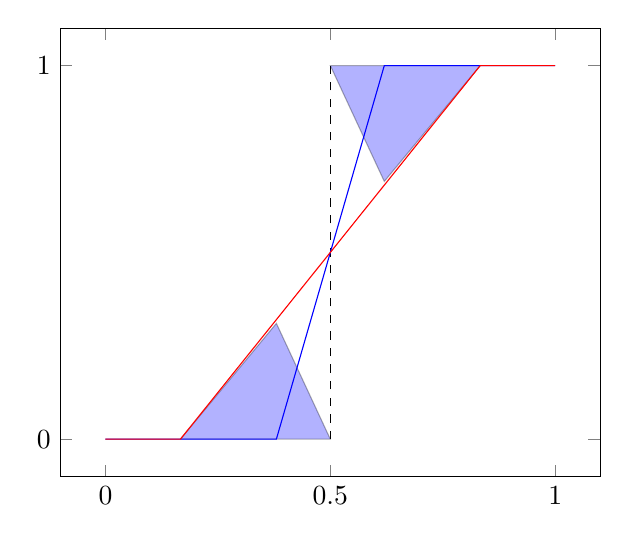
\begin{tikzpicture}
			\begin{axis}[legend pos=north west, legend style={fill=gray!10}, ytick={0, 1},xtick={0,0.5,1}]
				\addplot[dashed,black]coordinates{
					(0.5,0.0) (0.5, 1.0)
				};
				\addplot[fill=blue,opacity=0.3] coordinates{
				(.1666, 0.0)
 	 	 		(.38  , 0.31)
 	 	 		(.5, 0.0)
 	 	 		(.1666, 0.0)
				};
				\addplot[fill=blue,opacity=0.3] coordinates{
				(.8333, 1.0)
 	 	 		(.62  , 0.69)
 	 	 		(.5, 1.0)
 	 	 		(.8333, 1.0)
				};
				\addplot[color=blue] coordinates{
					(0,0)
					(.38  , 0.0)
					(.62  , 1.0)
					(1,1)
				};
				\addplot[color=red] coordinates{
					(0,0)
					(.166666, 0.0)
					(.833333, 1.0)
					(1,1)
				};
			\end{axis}
			\end{tikzpicture}
			}
			\end{center}
		\item $\left(\int_0^1|f_n - f_m|^p\right) \le \int_0^1|f_n - f_m|$, and so $\left(\int_0^1|f_n - f_m|^p\right)^\frac{1}{p} \le \left(\int_0^1|f_n - f_m|\right)^\frac{1}{p}$ for all $n, m$ and all $1 < p < \infty$. Therefore 
			$f_n$ is a Cauchy sequence. 
		\item The limit of the sequence in $L^p[0,1]$ for $1 \le p < \infty$ is going to be the 
			step function 
			\begin{equation*}
				f(x) = \left\{
					\begin{matrix} 
						0, & 0 \le x \le 0.5 \\ 
						1, & 0.5 \le x \le 1 
					\end{matrix}
					\right.
			\end{equation*} 
			(note that, being non-continuous, this limit is not 
			actually in the space $L^p$, but it is the limit of a sequence whose elements are in $L^p$) 
			\begin{center}
			\resizebox{0.38\textwidth}{!}{
			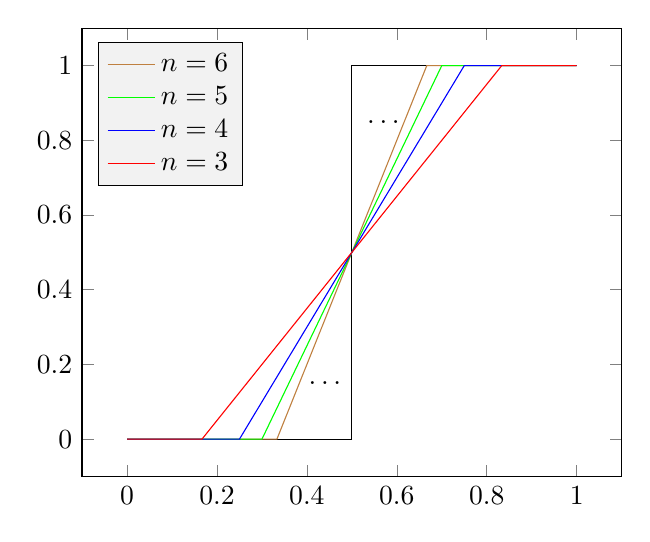
\begin{tikzpicture}
			\begin{axis}[legend pos=north west, legend style={fill=gray!10}]
				\addplot[color=black, forget plot] coordinates{
					(0,0)
					(.5, 0.0)
					(.5, 1.0)
					(1,1)
				};
				\addplot[color=brown] coordinates{
					(0,0)
					(.3333, 0.0)
					(.6666, 1.0)
					(1,1)
				};\addlegendentry{$n = 6$};
				\addplot[color=green] coordinates{
					(0,0)
					(.3, 0.0)
					(.7, 1.0)
					(1,1)
				};\addlegendentry{$n = 5$};
				\addplot[color=blue] coordinates{
					(0,0)
					(.25, 0.0)
					(.75, 1.0)
					(1,1)
				};\addlegendentry{$n = 4$};
				\addplot[color=red] coordinates{
					(0,0)
					(.166666, 0.0)
					(.833333, 1.0)
					(1,1)
				};\addlegendentry{$n = 3$};
				\draw (axis cs:0.44, 0.15) node {$\dots$};
				\draw (axis cs:0.57, 0.85) node {$\dots$};
			\end{axis}
			\end{tikzpicture}
			}
			\end{center}
	\end{enumerate}
%%%%%%%%%%%%%%%%%%%%%%%%%%%%%%%%%%%%%%%%%%%%%%%%%%%%%%%%%%%%%%%%%%%%%%%%%%%%%%%%%%%%%%%%%%%
\end{proof}
\end{pblm}

\pagebreak
\begin{pblm}~ %140
	\begin{enumerate}[(a)]
	\item Show that the sequence $\{f_n\}_{n=3}^\infty$ of the preceding problem is not 
		Cauchy in $L^\infty[0,1]$, or equivalently in $C[0,1]$ with the uniform norm. 
	\item Show that the limit $f$ from the preceding problem satisfies $\|f - f_n\|_\infty = 1/2$ 
		for each $n$. 
	\item Show that for any $g \in C[0,1]$, $\|f - g\|_\infty \ge 1/2$. (Thus $C[0,1]$ is not 
		dense in $L^\infty[0,1]$.)
	\end{enumerate}
\begin{proof}
	~
	\begin{enumerate}[(a)]
	\item Note that this part relies on part (b). 
		As the limit $f$ from the previous problem satisfies $\|f - f_n\|_\infty = 1/2$ for 
		all $n$, then for any $0 < \epsilon < 0.5$, for all $n$, $$\|f - f_n\| > \epsilon.$$ Thus 
		this sequence is not Cauchy in $L^\infty[0,1]$. 
	\item in $L^\infty[0,1]$, for each $n$, the value of $f_n$ at 0.5 is 0.5, and so 
		$\|f - f_n\|_\infty\ge 0.5$, but since this is the point at which 
		$f_n$ is furthest from $f$, we have $\|f - f_n\|_\infty = 0.5$ for all $n$. 
		\begin{center}
		\resizebox{0.38\textwidth}{!}{
		\begin{tikzpicture}
		\begin{axis}[legend pos=north west, legend style={fill=gray!10}, ytick={0, 1},xtick={0,0.5,1}]
			\addplot[color=black] coordinates{
				(0,0)
				(0.5, 0.0)
				(0.5, 1.0)
				(1,1)
			};
			\addplot[color=red] coordinates{
				(0,0)
				(.166666, 0.0)
				(.833333, 1.0)
				(1,1)
			};
		\end{axis}
		\end{tikzpicture}
		}
		\end{center}
	\item For any $g \in \C[0,1]$, we know that $\|f - g\|_\infty \le \frac{1}{2}$ in $[0, 0.5)$ implies that 
		$g(a) < \frac{1}{2}$ for at least one value $a \in [0,0.5)$, and similarly, 
		there is $b \in (0.5, 1]$ such that $g(b) > \frac{1}{2}$, and therefore by the intermediate value 
		theorem, there is some $a < c < b$ such that $g(c) = \frac{1}{2}$, and thus, since $f$ only takes values 
		$0$ and $1$ on the interval $[0,1]$, $\|f - g\|_\infty = \frac{1}{2}$
	\end{enumerate}
\end{proof}
\end{pblm}

\pagebreak
\begin{pblm} %141
	$L^\infty(E)$ is a Banach space. 
	%\\
	%{\scriptsize{(Let $\{f_n\}_{n=1}^\infty$ be a Cauchy sequence in $L^\infty(E)$ and choose a representative 
	%of each $f_n$, which we still denote by $f_n$. For each positive integer $k$ there is $n_k$ 
	%so that $\|f_n - f_m\|_\infty < 2^{-k}$ whenever $m, n \ge n_k$. Consider the sequence 
	%$\{f_{nk}\}_{k=1}^\infty$. Then $\ell > k$ implies $\|f_{n\ell}-f_{nk}\|<2^{-k}$. There is 
	%a set $A$, $m(A) = 0$, such that the series $f_{n_1}(x) + \sum\limits_{i=2}^k(f_{n_i}(x)-f_{n_{i-1}}(x))$ 
	%of real numbers converges absolutely for each $x\in E\setminus A$. The function $f$ defined as 
	%the pointwise limit of this series is in $L^\infty(E)$. Given $\epsilon > 0$ there is 
	%$n_\epsilon$ so that $m, n \ge n_\epsilon$ implies that $\|f_n - f_m\|_\infty < \epsilon$. Then 
	%for any such $f_m$ and any $x \in E\setminus A$, $|f(x) - f_m(x)| = 
	%\lim\limits_{k\to\infty}|f_{n_k}(x)-f_m(x)|\le\epsilon$.)}}
\begin{proof}
	We already know that $L^\infty(E)$ is a normed linear space, so all that remains to be shown 
	is that it is complete. (i.e. every Cauchy sequence converges)

	Let $\{f_n\}_{n=1}^\infty$ be a Cauchy sequence in $L^\infty(E)$, choose a representation of each 
	$f_n$, call it $f_n$. Then since $\{f_n\}_{n=1}^\infty$ is Cauchy, for any $k \in \Zp$, there is 
	a positive integer $n_k$ such that 
	\begin{equation*}
		||f_n - f_m||_\infty < \frac{1}{2^k}~~~\forall m, n \ge n_k
	\end{equation*}
	Then consider the sequence for $k > 0$ $\{f_{n_k}\}_{k=1}^\infty$. For any $l > k$, we know that 
	$||f_m - f_{n_l}||_\infty < \frac{1}{2^l} < \frac{1}{2^k}$ for all $m \ge n_l$, which implies that 
	$||f_{n_l} - f_{n_k}||_\infty < \frac{1}{2^k}$. 

	Then consider $F_k = f_{n_1} + \sum\limits_{n=2}^k (f_{n_i} - f_{n_{i-1}})$. Note that this is actually 
	another way of representing each $f_{n_k}$. Note that each $(f_{n_i} - f_{n_{i-1}})$ has 
	$||f_{n_i} - f_{n_{i-1}}||_\infty < \frac{1}{2^{i-1}}$, so 
	\begin{equation*}
		||F_{k+1} - F_k||_\infty < \frac{1}{2^k} ~~~\forall k
	\end{equation*}
	And furthermore, $||F_k||_\infty < ||f_{n_1}||_\infty + 1$ for all $k$. 
	So $F_k$ converges absolutely a.e., and if we define 
	\begin{equation*}
		\lim\limits_{k\to\infty}F_k = f
	\end{equation*}
	Then this is a bounded function a.e., and so $f \in L^\infty(E)$. 

	Now we need to show that $\{f_n\}_{n=1}^\infty$ converges to $f$. This is a Cauchy sequence, so 
	for any $\epsilon > 0$, there is $n_\epsilon$ such that for all $m, n \ge n_\epsilon$, 
	\begin{equation*}
		||f_n - f_m||_\infty < \epsilon
	\end{equation*}
	so for any such $f_m$, 
	\begin{equation*}
		|f(x) - f_m(x)| = \lim\limits_{n\to\infty}|f_{n_k}(x) - f_m(x)| \le \epsilon. 
	\end{equation*}
	So $\{f_n\} \rightarrow f$ a.e. and $f \in L^\infty(E)$ for any Cauchy sequence inf $L^\infty(E)$. 
	Thus $L^\infty(E)$ is a complete (and therefore Banach) space. 
\end{proof}
\end{pblm}

\begin{pblm}%142
	For each $1\le p < \infty$, if $\{f_n\}_{n=1}^\infty$ is a Cauchy sequence in $L^p(E)$ and 
	if we choose a representative of each $f_n$ (we will still denote these functions by $\{f_n\}$), 
	then there is a subsequence $\{f_{n_k}\}_{k=1}^\infty$ that converges pointwise a.e. on $E$ to 
	a measurable function $f$ such that $\int_E|f|^p < \infty$. 
	%{\scriptsize{(For each positive integer $k$ there 
	%is $n_k$ so that $\|f_n - f_m\|_p < 2^{-k}$ whenever $m,n \ge n_k$. Why? Consider the sequence 
	%$\{f_{n_k}\}_{k=1}^\infty$. Then $\ell > k$ implies $\|f_{n_\ell} - f_{n_k}\|_p < 2^{-k}$. 
	%For each integer $k \ge 2$, set $g_k = |f_{n_1}| + \sum\limits_{i=2}^k|f_{n_i} - f_{n_{i-1}}|$. 
	%Then $\{g_k\}_{k=1}^\infty$ is a non-decreasing sequence of non-negative functions such that 
	%$\|g_k\|_p \le \|f_{n_1}\|_p + 1$ for each $k$, and the extended real-valued function 
	%$g(x) = \lim\limits_{k\to\infty}g_k(x)$ satisfies $\int_Eg^p = \lim\limits_{k\to\infty}\int_Eg^p_k < \infty$. 
	%For almost all $x \in E$, the series $f_{n_1}(x) + \sum\limits_{i=2}^\infty(f_{n_i}(x) - f_{n_{i-1}}(x))$ 
	%of real numbers converges absolutely, and so defines a measurable  function $f$ there. This 
	%function is in $L^p(E)$.)}}
\begin{proof}
	Let $1 \le p < \infty$. Then if $\{f_n\}_{n=1}^\infty$ is Cauchy, then for any $k \in \Zp$, 
	there is $n_k$ such that 
	\begin{equation*}
		||f_n - f_m||_p , \frac{1}{2^k} ~~ \forall m, n \ge n_k
	\end{equation*}

	Now consider the subsequence $\{f_{n_k}\}_{k=1}^\infty$ of $\{f_n\}$. As in the 
	previous problem, for any $l > k$, $||f_{n_l} - f_{n_k}||_\infty < \frac{1}{2^k}$. 
	Now, for each $k \ge 2$, let 
	\begin{equation*}
		g_k(x) = |f_{n_1}| + \sum\limits_{i=2}^k|f_{n_i} - f_{n_{i-1}}|
	\end{equation*}
	Then $\{g_k\}_{k=2}^\infty$ is non-decreasing, non-negative, and 
	since for each $k$, $|g_k| \le |f_{n_1}| + 1$, then 
	\begin{equation*}
		||g_k||_p \le ||f_{n_1}||_p + 1
	\end{equation*}
	for each $k$, and setting $g = \lim\limits_{k\to\infty}g_k$, we have 
	\begin{equation*}
		\int_Eg^p = \lim\limits_{k\to\infty}\int_Eg^p_k < \infty
	\end{equation*}

	This sequence converges absolutely, and if we let 
	\begin{equation*}
		f = \lim\limits_{k\to\infty}\left\{f_{n_1} + \sum\limits_{i=2}^k(f_{n_i} - f_{n_i - 1})\right\}
	\end{equation*}
	then we know that this sequence converges absolutely, and as each term $f_k$ is bounded by $g_k$, we have 
	$|f| \le g$ which implies that 
	\begin{equation*}
		\int_E|f|^p \le \int_Eg^p < \infty
	\end{equation*}
	and so $f$ is in $L^p(E)$. 
\end{proof}
\end{pblm}

\begin{pblm}%143
	If $\{f_n\}_{n=1}^\infty$ and $f$ are as in the preceding problem, then $f_n \rightarrow f$ in 
	$L^p(E)$. Thus $L^p(E)$ is complete.\\
	{\scriptsize{(Let $\epsilon > 0$ be given. For $m,n > n_\epsilon$ Then Fatou's Lemma implies 
	$ \int_E|f-f_m|^p \le \lim\inf\limits_{k}\int_E|f_{n_k} - f_m|^p < \epsilon^p.) $ }}
\begin{proof}
	Let $\{f_n\}_{n=1}^\infty$ and $f$ be as in the previous problem. Then since $\{f_n\}$ is 
	Cauchy, for any $\epsilon > 0$, 
	\begin{equation*}
		||f_n - f_m||_p < \epsilon ~~~ m, n \ge n_\epsilon
	\end{equation*}
	so by Fatou's Lemma (\mPref{p:fatou}), 
	\begin{equation*}
		\int_E |f - f_m|^p \le \lim\inf\limits_{k}\int_E|f_{n_k} - f_m|^p 
				= \lim\inf\limits_{k}||f_{n_k} - f_m||_p < \epsilon^p
	\end{equation*}
	and so the sequence $\{f_n\}_{n=1}^\infty$ converges to $f$. 
\end{proof}
\end{pblm}

\begin{rmk}%144
	The completeness of $L^p$ is sometimes referred to as the Riesz-Fischer Theorem, although 
	what Riesz actually proved in 1906 was rather different. It was similar to the example 
	explored below. 
\end{rmk}

\begin{rmk}%145
	There is another way to arrange the proof of the completeness of $L^p$ that looks a little 
	slicker, but perhaps changes the perception of what's really going on. One proves the abstract 
	theorem that a normed linear space $X$ is complete if and only if the following property is 
	true: if a series $\sum\limits_{n=1}^\infty x_n$ \textbf{converges absolutely} (this means 
	that the series $\sum\limits_{n=1}^\infty \|x_n\|$ of norms converges in $\R$) then the series 
	converges in $X$ (this means that the sequence of partial sums $\sum\limits_{n=1}^N x_n$ 
	converges to an element of $X$). Then you show that $L^p(E)$ has this property. If you look 
	carefully, you will find these elements in what we did.
\end{rmk}

\begin{defn}%146
	The set $\ell^p$ (read ``little $L^p$'') is the set of real (or complex) sequences $\{c_n\}_{n=1}^\infty$ 
	such that $\sum\limits_{n=1}^\infty |c_n|^p < \infty$. It is a complete normed linear space-a 
	Banach space-with the norm 
	\begin{equation*}
		\|\{c_n\}\|_p = \left(\sum\limits_{n=1}^\infty |c_n|^p\right)^{1/p}. 
	\end{equation*}
	(That this is a norm with respect to which $\ell^p$ is complete can be proved by methods 
	roughly similar to what we have done.)
\end{defn}

\begin{rmk}%147
	We can add more structure for $L^2$ and $\ell^2$. An \textbf{inner product} on a vector 
	space is a map $(\cdot , \cdot): V \times V \rightarrow \R$ with the properties 
	\begin{enumerate}
	\item $(v,v) \ge 0$ and $(v, v) = 0$ iff $v = 0$ (zero element in $V$, of course), 
	\item $(v,w) = (w,v)$ for all $v, w\in V$, 
	\item $(av + bw, u) = a(v,u) + b(w, u)$ for all $u, v, w \in V$ and all $a, b \in \R$. 
	\end{enumerate}
	Given an inner product, $\|v\| = \sqrt{(v,v)}$ is a norm on $V$, so every inner product 
	space is a normed linear space and hence a metric space. (Topology from algebra!) If it is 
	complete as a metric space, we call it a \textbf{Hilbert space}. However in an inner product 
	space we can also define the angle between elements by analogy with the dot product. In 
	particular $v$ and $w$ are \textbf{orthogonal} if $(v,w) = 0$. It is possible to extend 
	``dot product geometry'' to this context-orthogonal bases, expressing an arbitrary element 
	as the sum of its projections onto the elements of an orthogonal basis and so forth. The so 
	forth includes the equivalent of the Pythagorean Theorem: the square of the norm of an element 
	is the sum of the squares of the lengths of its projections. However the extension must 
	cope with the fact that bases are typically countably infinite sets, so the sums are infinite 
	sums and there are questions of convergence.

	In $\ell^2$ the inner product is $(\{c_n\}, \{d_n\}) = \sum\limits_{n=1}^\infty c_nd_n$. The 
	equivalent of H\"{o}lder's Inequality guarantees that $|(\{c_n\},\{d_n\})| \le \|\{c_n\}\|\|\{d_n\}\|$ 
	and so in particular that the sum converges absolutely. In $L^2(E)$ the inner product is 
	$(f,g) = \int_Efg$. Again this converges by H\"{o}lder's Inequality. 

	In $L^2[0,\pi]$ the sequence $\{\sin nx\}_{n=1}^\infty$ has the properties 
	$\|\sin nx\|_2 = \sqrt{\frac{\pi}{2}}$ and $\sin nx \perp \sin mx$ if $m \neq n$, that is, 
	$\int_0^\pi \sin nx \sin mx dx = 0$ if $m neq n$. The projection of any function $f \in L^2[0,\pi]$ 
	on $nx$ is 
	\begin{equation*}
		\frac{(f,\sin nx)}{(\sin nx, \sin nx)}\sin nx = 
		\left(\frac{2}{\pi}\int_0^\pi f(t) \sin nt dt\right)\sin nx. 
	\end{equation*}
	The projection $p_n$ of $f \in L^2[0,\pi]$ on SPAN$\{\sin x, \sin 2x, \dots \sin nx\}$ is 
	$\sum\limits_{k=1}^n c_k\sin kx$ where $c_k = \frac{2}{\pi}\int_0^\pi f(t) \sin kl dt$. It is 
	easy to see, using the orthogonality of the different sine functions that $\|p_n\|_2^2 = 
	\sum\limits_{k=1}^nc_k^2 \le \|f\|_2^2$ where the last inequality just comes from the fact that 
	any projection of $f$ has norm less than or equal to that of $f$. It follows that $\{c_k\}_{k=1}^\infty$ 
	is in $\ell^2$, that $\{p_n\}_{n=1}^\infty$ is Cauchy in $L^2[0,\pi]$ (since $\|p_n - p_m\|_2^2 = 
	\sum\limits_{k=m+1}^nc_k^2$), and then by completeness that $\{p_n\}_{n=1}^\infty$ converges 
	in $L^2[0,\pi]$ to an element $\sum\limits_{k=1}^\infty c_k\sin kx$. It turns out that 
	$f = \sum\limits_{k=1}^\infty c_k \sin kx$ and that 
	\begin{equation*}
		\|f\|_2^2 = \sum\limits_{k=1}^\infty c_k^2  = \|\{c_n\}\|^2. 
	\end{equation*}
	(These turn out to be equivalent to the statement that the only element of $L^2[0,\pi]$ that 
	is orthogonal to every $\sin nx$ is the zero element, that is, the set $\{\sin nx\}_{n=1}^\infty$ 
	is \textbf{complete} (roughly, large enough to function as a basis).)

	The result of all of this is that the mapping $f\rightarrow \{c_n\}$ is an isometry (linear 
	mapping preserving the norm) of $L^2[0,\pi]$ onto $\ell^2$. In particular, given any 
	sequence in $\ell^2$, there is an $L^2$ function $f$ with that sequence of Fourier sine coefficients. 
	This is approximately the content of the original Riesz-Fischer Theorem in 1906.
\end{rmk}
